\documentclass[leqno]{article}
\usepackage{float}
\usepackage[brazil]{babel} %\usepackage[latin1]{inputenc}
\usepackage{a4wide}
\setlength{\oddsidemargin}{-0.2in}
% % \setlength{\oddsidemargin}{0.2in}
\setlength{\evensidemargin}{-0.2in}
% % \setlength{\evensidemargin}{0.5in}
% % \setlength{\textwidth}{5.5in}
\setlength{\textwidth}{6.5in}
\setlength{\topmargin}{-1.2in}
\setlength{\textheight}{10in}
\usepackage[]{amsfonts} \usepackage[]{amsmath}
\usepackage[]{amssymb} \usepackage[]{latexsym}
\usepackage{graphicx,color} \usepackage{amsthm}
\usepackage{mathrsfs} \usepackage{url}
\usepackage{cancel} \usepackage{enumerate}
\usepackage{xifthen} \usepackage{tikz}
\usetikzlibrary{automata,arrows,positioning,calc}
\usepackage{listings}

\numberwithin{equation}{section}

\setlength{\parindent}{12 pt}

\begin{document}
	
	\newtheorem{teo}{Teorema}[section] \newtheorem*{teo*}{Teorema}
	\newtheorem{prop}[teo]{Proposição} \newtheorem*{prop*}{Proposição}
	\newtheorem{lema}[teo]{Lemma} \newtheorem*{lema*}{Lema}
	\newtheorem{cor}[teo]{Corolário} \newtheorem*{cor*}{Corolário}
	
	\theoremstyle{definition}
	\newtheorem{defi}[teo]{Definição} \newtheorem*{defi*}{Definição}
	\newtheorem{exem}[teo]{Exemplo} \newtheorem*{exem*}{Exemplo}
	\newtheorem{obs}[teo]{Observação} \newtheorem*{obs*}{Observação}
	\newtheorem*{hipo}{Hipóteses}
	\newtheorem*{nota}{Notação}
	
	\newcommand{\ds}{\displaystyle} \newcommand{\nl}{\newline}
	\newcommand{\eps}{\varepsilon} \newcommand{\ssty}{\scriptstyle}
	\newcommand{\bE}{\mathbb{E}}
	\newcommand{\cB}{\mathcal{B}}
	\newcommand{\cF}{\mathcal{F}}
	\newcommand{\cA}{\mathcal{A}}
	\newcommand{\cM}{\mathcal{M}}
	\newcommand{\cD}{\mathcal{D}}
	\newcommand{\cN}{\mathcal{N}}
	\newcommand{\cL}{\mathcal{L}}
	\newcommand{\cLN}{\mathcal{LN}}
	\newcommand{\bP}{\mathbb{P}}
	\newcommand{\bQ}{\mathbb{Q}}
	\newcommand{\bN}{\mathbb{N}}
	\newcommand{\bR}{\mathbb{R}}
	\newcommand{\bZ}{\mathbb{Z}}
	
	\newcommand{\bfw}{\mathbf{w}}
	\newcommand{\bfv}{\mathbf{v}}
	\newcommand{\bfu}{\mathbf{u}}
	\newcommand{\bfx}{\mathbf{x}}
	\newcommand{\bfb}{\mathbf{b}}
	
	\newcommand{\bvecc}[2]{%
		\begin{bmatrix} #1 \\ #2  \end{bmatrix}
	}
	\newcommand{\bveccc}[3]{%
		\begin{bmatrix} #1 \\ #2 \\ #3  \end{bmatrix}
	}
	
	\newenvironment{sol} 
	{
		\vspace{4mm}
		\noindent\textbf{Resolução:}
		\strut\newline
		\smallskip
		\hspace{-3.5mm} 
	} 
	% Objetos que aparecem *após* o ambiente. 
	% (você pode, por exemplo, modificar, 
	% ou remover, a barra horizontal} 
	%{\noindent\rule{4cm}{.1mm}}
	
	
	\title{Álgebra Linear - Aula Prática 1}
	
	\author{Iara Cristina Mescua Castro}
	
	\date{\today}
	
	\maketitle
	
	\begin{enumerate}
		
		%%%%%%%%%%%%%%%%%%%%%%%%%%%%%%%%%%%%%%%%%%%%%%%%%%%%%%%%%
		%%%%%%%%%%%%%%%%%%%%%% Exercício 1 %%%%%%%%%%%%%%%%%%%%%%
		%%%%%%%%%%%%%%%%%%%%%%%%%%%%%%%%%%%%%%%%%%%%%%%%%%%%%%%%%
		
		\item  Teste a função dada usando algumas matrizes quadradas A e respectivos 
		vetores b. Use exemplos dos quais você saiba a resposta para verificar se a 
		função realmente está funcionando corretamente.
		
		\begin{sol}
			$$A = \begin{bmatrix}
				3 & 1 & -1\\
				1 & -1 & 1\\
				2 & 1 & 1
			\end{bmatrix}  b = \begin{bmatrix}
				1 \\
				-3 \\
				0
			\end{bmatrix} $$

		Resolvendo por eliminação de Gauss:
		
		$$\begin{bmatrix}
			3 & 1 & -1 & | & 1\\
			1 & -1 & 1 & | & -3\\
			2 & 1 & 1 & | & 0
		\end{bmatrix}$$
	
		$R_1 \longleftrightarrow R_2$
		$$\begin{bmatrix}
			1 & -1 & 1 & | & -3\\
			3 & 1 & -1 & | & 1\\
			2 & 1 & 1 & | & 0
		\end{bmatrix}$$
		
		$-3R_1 + R_2 \longleftrightarrow R_2$
		$$\begin{bmatrix}
			1 & -1 & 1 & | & -3\\
			0 & 4 & -4 & | & 10\\
			2 & 1 & 1 & | & 0
		\end{bmatrix}$$
		
		$-2R_1 + R_3 \longleftrightarrow R_3$
		$$\begin{bmatrix}
			1 & -1 & 1 & | & -3\\
			0 & 4 & -4 & | & 10\\
			0 & 3 & -1 & | & 6
		\end{bmatrix}$$
	
		$R_2/4 \longleftrightarrow R_2$
		$$\begin{bmatrix}
			1 & -1 & 1 & | & -3\\
			0 & 1 & -1 & | & \frac{10}{4}\\
			0 & 3 & -1 & | & 6
		\end{bmatrix}$$
	
		$R_2 + R_1 \longleftrightarrow R_1$
		$$\begin{bmatrix}
			1 & 0 & 0 & | & -\frac{1}{2}\\
			0 & 1 & -1 & | & \frac{5}{2}\\
			0 & 3 & -1 & | & 6
		\end{bmatrix}$$
	
		$-3R_2 + R_3 \longleftrightarrow R_3$
		$$\begin{bmatrix}
			1 & 0 & 0 & | & -\frac{1}{2}\\
			0 & 1 & -1 & | & \frac{5}{2}\\
			0 & 0 & 2 & | & -\frac{3}{2}
		\end{bmatrix}$$
	
		$R_3/2 \longleftrightarrow R_3$
		$$\begin{bmatrix}
			1 & 0 & 0 & | & -\frac{1}{2}\\
			0 & 1 & -1 & | & \frac{5}{2}\\
			0 & 0 & 1 & | & -\frac{3}{4}
		\end{bmatrix}$$
	
		$R_3 + R_2 \longleftrightarrow R_2$
		$$\begin{bmatrix}
			1 & 0 & 0 & | & -\frac{1}{2}\\
			0 & 1 & 0 & | & \frac{7}{4}\\
			0 & 0 & 1 & | & -\frac{3}{4}
		\end{bmatrix}$$
	
		Temos que:
		$$x = \begin{bmatrix}
			-\frac{1}{2} \\
			\frac{7}{4} \\
			-\frac{3}{4}
		\end{bmatrix} = \begin{bmatrix}
		-0.5 \\
		1.75 \\
		-0.75
		\end{bmatrix}$$
	
		Decomposição LU de A:
		
		$$\begin{bmatrix}
			3 & 1 & -1 \\
			1 & -1 & 1 \\
			2 & 1 & 1 
		\end{bmatrix}$$
	
		$R_2 \longleftrightarrow R_2 - \frac{1}{3}R_1$
			$$\begin{bmatrix}
				3 & 1 & -1 \\
				0 & -\frac{4}{3} & \frac{4}{3} \\
				2 & 1 & 1 
			\end{bmatrix}$$
		
		$R_3 \longleftrightarrow R_3 - \frac{2}{3}R_1$
			$$\begin{bmatrix}
				3 & 1 & -1 \\
				0 & -\frac{4}{3} & \frac{4}{3} \\
				0 & \frac{1}{3} & \frac{5}{6} 
			\end{bmatrix}$$
		
		$R_3 \longleftrightarrow R_3 + \frac{1}{4}R_2$
			$$U = \begin{bmatrix}
				3 & 1 & -1 \\
				0 & -\frac{4}{3} & \frac{4}{3} \\
				0 & 0 & 2
			\end{bmatrix} = \begin{bmatrix}
				3 & 1 & -1 \\
				0 & -1.333333 & 1.3333333 \\
				0 & 0 & 2
			\end{bmatrix}$$
		
			$$L = \begin{bmatrix}
				1 & 0 & 0 \\
				\frac{1}{3} & 1 & 0 \\
				\frac{2}{3} & -\frac{1}{4} & 1
			\end{bmatrix} = \begin{bmatrix}
			1 & 0 & 0 \\
			0.33 & 1 & 0 \\
			0.66 & -0.25 & 1
			\end{bmatrix}$$
		
			$$C = \begin{bmatrix}
				3 & 1 & -1 \\
				0.33 & -1.33 & 1.33 \\
				0.66 & -0.25 & 2
			\end{bmatrix} $$
		
	
		Conferindo no Scilab, verificamos que a função está operando corretamente para este exemplo.
		\begin{figure}[H]
			\centering
			\includegraphics[width=0.45\linewidth]{q1}
		\end{figure}
		
\end{sol}

%%%%%%%%%%%%%%%%%%%%%%%%%%%%%%%%%%%%%%%%%%%%%%%%%%%%%%%%%
%%%%%%%%%%%%%%%%%%%%%% Exercício 2 %%%%%%%%%%%%%%%%%%%%%%
%%%%%%%%%%%%%%%%%%%%%%%%%%%%%%%%%%%%%%%%%%%%%%%%%%%%%%%%%

\item Agora teste com a matriz: $A1 = [1\quad -2 \quad 5 \quad 0; 2 \quad -4 \quad 1 \quad 3; -1 \quad 1 \quad 0 \quad 2; 0 \quad 3 \quad 3 \quad 1]$ e com o vetor $b1=[1;0;0;0]$.

\begin{sol}

	\begin{figure}[H]
		\centering
		\includegraphics[width=0.4\linewidth]{q2}
	\end{figure}
	
Houve um erro, pois na quarta linha teremos um elemento nulo, que conflita com a divisão pelo pivô $A(j,j)$ na função.
\end{sol}

%%%%%%%%%%%%%%%%%%%%%%%%%%%%%%%%%%%%%%%%%%%%%%%%%%%%%%%%%
%%%%%%%%%%%%%%%%%%%%%% Exercício 3 %%%%%%%%%%%%%%%%%%%%%%
%%%%%%%%%%%%%%%%%%%%%%%%%%%%%%%%%%%%%%%%%%%%%%%%%%%%%%%%%

\item Modifique a função dada trocando linhas quando no início da iteração j o 
elemento na posição (j,j) é nulo. Chame esta nova função de 
$Gaussian\_Elimination\_2$ e teste-a com a matriz A1 e o vetor b1 dados.
Agora teste-a com a matriz $A2=[0 \quad 10^{-20} \quad 1; 10^{-20} \quad 1 \quad 1; 1 \quad 2 \quad 1]$ e o vetor $b2=[1; 0; 0]$.

\begin{sol}
	\begin{lstlisting}[language=Scilab]
		function [x, C]=Gaussian_Elimination_2(A, b) 
		C=[A,b];   
		[n]= length(b); 
		
		for j=1:(n-1)
			if C(j,j) == 0	
				diff_zero = find(C(:,j));
				x = diff_zero(diff_zero>j);
				C([j x(1)],:) = C([x(1) j],:);	
			end
			for i=(j+1):n 
				C(i,j)=C(i,j)/C(j,j); 
				C(i,j+1:n+1)=C(i,j+1:n+1)-C(i,j)*C(j,j+1:n+1); 				
			end 
		end 
			
		x=zeros(n,1); 		
		
		// Calcula x, sendo Ux=C(1:n,n+1) 
		
		x(n)=C(n,n+1)/C(n,n); 
		for i=n-1:-1:1 
			sum = b(i);
			for k=i+1:n
				sum = sum-A(i,j)*x(k);
			end
			x(i) = sum/A(i,i); 
		end 
		
		C=C(1:size(C,1),1:size(C,1)); 
		
		endfunction
	\end{lstlisting}

	Com a nova função, dentro do loop há uma nova condição que quando encontra $C(j,j)$ igual a 0, verifica as linhas da matriz que tem um número diferente de 0 naquela coluna j com a função $find()$ e depois encontra qual dessas linhas é a próxima depois da linha j, para então, realizar a troca de linhas toda vez que durante o loop encontrarmos um 0 no pivô na diagonal.
	
	Testando com a matriz $A_1$ e $b_1$:
	
	\begin{figure}[H]
		\centering
		\includegraphics[width=0.45\linewidth]{q3_pt1}
	\end{figure}

	
	Podemos verificar a diferença através do comando de divisão de matrizes que está funcionando corretamente: 
	\begin{figure}[H]
		\centering
		\includegraphics[width=0.25\linewidth]{A1-b1}
	\end{figure}
	\newpage
	Testando com a matriz $A2=[0 \quad 10^{-20} \quad 1; 10^{-20} \quad 1 \quad 1; 1 \quad 2 \quad 1]$ e o vetor $b2=[1; 0; 0]$, temos:
	\begin{figure}[H]
		\centering
		\includegraphics[width=0.5\linewidth]{A2-b2}
	\end{figure}
	
\end{sol}

Mesmo sem erros na execução, a solução está incorreta. Podemos verificar a diferença através do comando de divisão de matrizes:

	\begin{figure}[H]
		\centering
		\includegraphics[width=0.3\linewidth]{result-A2}
	\end{figure}

%%%%%%%%%%%%%%%%%%%%%%%%%%%%%%%%%%%%%%%%%%%%%%%%%%%%%%%%%
%%%%%%%%%%%%%%%%%%%%%% Exercício 4 %%%%%%%%%%%%%%%%%%%%%%
%%%%%%%%%%%%%%%%%%%%%%%%%%%%%%%%%%%%%%%%%%%%%%%%%%%%%%%%%

\item Modifique a função do item 3 para escolher o maior pivô em módulo quando 
no  início  da  iteração  j  o  elemento  na  posição  $(j,j)$  é  nulo.  Chame  esta  nova 
função  de  $Gaussian\_Elimination\_3$  e  teste-a  com  a  matriz  $A2$  e  o  vetor  $b2$ 
dados.  Agora  com  a  matriz  $A3=[10^{-20} \quad 10^{-20} \quad 1; 10^{-20} \quad 1 \quad 1; 1 \quad 2 \quad 1]$ e o vetor $b3=b2$.
\begin{sol}
	\begin{lstlisting}[language=Scilab]
		function [x, C]=Gaussian_Elimination_3(A, b) 
		C=[A,b];   
		[n]= length(b); 
		
		for j=1:(n-1)
			if C(j,j) == 0	
				x = L(:,j);
				x = (max(abs(x))); 
				index = find(L(:,j) == x);
				L([j index(1)],:) = L([index(1) j],:);
				C([j index(1)],:) = C([index(1) j],:);
			end
			for i=(j+1):n 
				C(i,j)=C(i,j)/C(j,j); 
				C(i,j+1:n+1)=C(i,j+1:n+1)-C(i,j)*C(j,j+1:n+1); 
			end 
		end 
		
		x=zeros(n,1); 
		
		// Calcula x, sendo Ux=C(1:n,n+1) 
		
		x(n)=C(n,n+1)/C(n,n); 
		for i=n-1:-1:1 
			sum = b(i);
			for k=i+1:n
				sum = sum-A(i,j)*x(k);
			end
			x(i) = sum/A(i,i); 
		end 
		
		C=C(1:size(C,1),1:size(C,1)); 
		
		endfunction
	\end{lstlisting}
	Agora não precisamos apenas do índice, mas do seu elemento correspondente que será o maior pivô para a troca de linhas. Para isso, indexamos eles na matriz para visualizar os valores e devolvemos o $max()$ (função que pega o valor máximo de uma matriz) do módulo desse vetor $abs()$ x. Agora temos o maior valor, então criamos uma condição com $find(C(:,j) == x)$ para ver qual a linha desse valor e por fim, fazer a troca.
	
	Esta simples mudança oferece mais estabilidade para a função.

	Testando com  a  matriz  $A2$ e o vetor $b2$, agora teremos a solução correta.
	
	\begin{figure}[H]
		\centering
		\includegraphics[width=0.5\linewidth]{A2-b2correto}
	\end{figure}
	
	Testando com a matriz $A3=[10^{-20} \quad 10^{-20} \quad 1; 10^{-20} \quad 1 \quad 1; 1 \quad 2 \quad 1]$ e o vetor $b3=b2$:
	
	\begin{figure}[H]
		\centering
		\includegraphics[width=0.4\linewidth]{A3-b3teste}
	\end{figure}

	Mesmo sem erros na execução, a solução está incorreta. Podemos verificar a diferença através do comando de divisão de matrizes:
	
	\begin{figure}[H]
		\centering
		\includegraphics[width=0.2\linewidth]{"A3-b3"}
	\end{figure}
	
	

\end{sol}

%%%%%%%%%%%%%%%%%%%%%%%%%%%%%%%%%%%%%%%%%%%%%%%%%%%%%%%%%
%%%%%%%%%%%%%%%%%%%%%% Exercício 5 %%%%%%%%%%%%%%%%%%%%%%
%%%%%%%%%%%%%%%%%%%%%%%%%%%%%%%%%%%%%%%%%%%%%%%%%%%%%%%%%

\item Modifique a função do item 4 para escolher sempre o maior pivô em módulo
no início da iteração j independente do elemento na posição (j,j) ser nulo ou
não. Nessa função, retorne também a matriz de permutação P utilizada.
Chame esta nova função de $Gaussian\_Elimination\_4$ e teste-a com a matriz
A3 e o vetor b3 dados.

\begin{sol}
	A mudança é simples, basta remover as linhas da condição de $C(j,j)$ ser nulo ou
	não. O erro será solucionado, devemos fazer a troca de linhas com valores muito próximos a zero, o que não acontecia originalmente, mas com a nova função a  troca de linhas será feita de qualquer forma para o maior pivô em módulo, evitando erros de aproximação.
	
	\begin{lstlisting}[language=Scilab]
		function [x, C]=Gaussian_Elimination_4(A, b) 
		C=[A, b];
		[n]=size(C, 1);
		P = eye(n, n);
		for j = 1:(n - 1)
		// O pivo esta na posicao (j,j)
		p_col = abs(C(j:n, j));
		// Extrai os valores absolutos da coluna pivo atual
		// em linhas maiores que a atual
		[m, i] = max(p_col);
		// Encontra onde ela tem seu valor maximo
		i = i + j - 1
		if i > j
		P([j i], :) = P([i j], :);
		C([j i], :) = C([i j], :);
		// Reordena as linhas se a atual nao tem o maior valor
		end
		for i = (j + 1):n
		// O elemento C(i,j) eh o elemento na posicao (i, j) de L
		// na decomposicao LU de A
		C(i, j) = C(i, j) / C(j, j);
		// Linha i <- Linha i - C(i, j) * Linha j
		// Somente os elementos da diagonal ou acima sao computados
		// (aqueles que compoem a matrix U)
		C(i, j+1:n+1)=C(i, j+1:n+1) - C(i, j) * C(j, j+1:n+1);
		end
		end
		x = zeros(n, 1);
		// Calcula x, sendo Ux=C(1:n,n+1)
		x(n) = C(n, n+1) / C(n, n);
		for i = n-1:-1:1
		x(i) = (C(i, n+1) - C(i, i:n) * x(i:n)) / C(i, i);
		end
		C = C(1:n, 1:n);
		endfunction
	\end{lstlisting}

	Testando com a matriz $A3$ e o vetor $b3$, teremos:
	\begin{figure}[H]
		\centering
		\includegraphics[width=0.6\linewidth]{q5}
	\end{figure}
	
	Agora a solução está correta.
	\begin{figure}[H]
		\centering
		\includegraphics[width=0.3\linewidth]{q5-correto}
	\end{figure}

\end{sol}

%%%%%%%%%%%%%%%%%%%%%%%%%%%%%%%%%%%%%%%%%%%%%%%%%%%%%%%%%
%%%%%%%%%%%%%%%%%%%%%% Exercício 6 %%%%%%%%%%%%%%%%%%%%%%
%%%%%%%%%%%%%%%%%%%%%%%%%%%%%%%%%%%%%%%%%%%%%%%%%%%%%%%%%

\item Uma vez que você tem a decomposição LU de uma matriz quadrada A de
ordem n (ou de PA, sendo P uma matriz permutação) a resolução de um
sistema linear Ax=b pode ser obtida mais rapidamente usando a
decomposição LU já feita, em vez de fazer todo o escalonamento de novo.
Escreva uma função Scilab de nome $Resolve\_com\_LU$, que receba como
variáveis de entrada uma matriz C com a decomposição LU de A (ou de PA,
conforme matriz retornada pelas funções anteriores) e uma matriz B de
ordem n x m e retorne uma matriz X, com a mesma ordem de B, cujas
colunas sejam as soluções dos sistemas lineares $A_xi=bi$.
Observação: talvez você ache necessário passar outra(s) variável(is) de
entrada para essa função.
Teste a sua função com a matriz A1 dada anteriormente e com a matriz
$B1=[2 4 -1 5 ;0 1 0 3 ; 2 2 -1 1 ; 0 1 1 5 ]$. Teste também com a matriz A2
dada anteriormente e com a matriz $B2=[1 1 2; 1 -1 0; 1 0 1]$. Finalmente, teste
com a matriz A3 dada anteriormente e com a matriz B3=B2.


\begin{sol}
	\begin{lstlisting}[language=Scilab]
		function X=Resolve_com_LU(C, B, P)
		B = P*B;
		m = size(B,2); //colunas de B
		n = size(C,1); //linhas
		L = tril(C); //Matriz L (triangular inferior)
		L(boolean(eye(n)))=1;
		U = triu(C); //Matriz U (triagular superior)
		X = zeros(n,m);
		
		for k = 1:m
		b_i = B(1:n, k); //vetores b_i
		y_i = resolveL(L,b_i); //vetores y_i
		x_i = resolveU(U,y_i); //x_i = U\y_i
		X(1:n, k) = x_i; //x_i em X
		end
		endfunction
		
		//Ly = b
		function y = resolveL(L,b)
		n = size(L,1);
		m = size(b,1);
		y = zeros(m,1);
		y(1) = b(1)/L(1,1);
		for i=2:n
		y(i) = (b(i) - L(i,1:i-1)*y(1:i-1))/L(i,i);
		end
		endfunction
		
		//Ux = y
		function x = resolveU(U,y)
		n = size(U,1);
		x = zeros(n,1);
		x(n) = y(n)/U(n,n);
		for i=n-1:-1:1
		x(i) = (y(i) - U(i,1:i-1)*x(1:i-1))/U(i,i);
		end
		endfunction
	\end{lstlisting}

Nessa função, recebemos a matriz $C, B e P$. Primeiro usamos a matriz de permutação P para $B = P * B$ e separamos a matriz C ela nas duas matrizes $L$ e $U$ com o comando $tril()$ e $triu()$. Depois, criamos duas funções a parte para resolver o seguinte sistema:

$$Ax = b$$
Sabendo que $A = LU$
$$LUx = b$$
$$L(Ux) = b$$
Chamamos $Ux = y$
Substituindo:
$$Ly = b$$
Então ficamos com essas duas equações: $Ux = y$ e $Ly = b$. Resolvemos ela com as funções $resolveL(L,b)$ e $resolveU(U,y)$ e por último, chamamos essas funções em um loop na função inicial para encontrar as soluções dos sistemas lineares $Ax_i = b_i$ e armazenamos elas na matriz $X$.

Testando com todas as matrizes:
\begin{figure}[H]
	\centering
	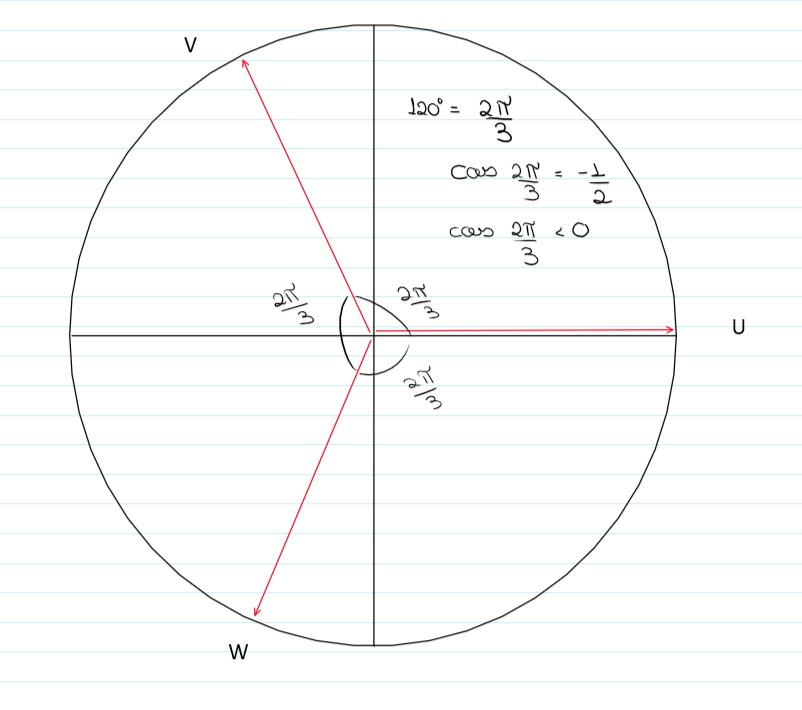
\includegraphics[width=0.5\linewidth]{6.1}
	\caption{A1}
	\label{fig:6}
\end{figure}

\begin{figure}[H]
	\centering
	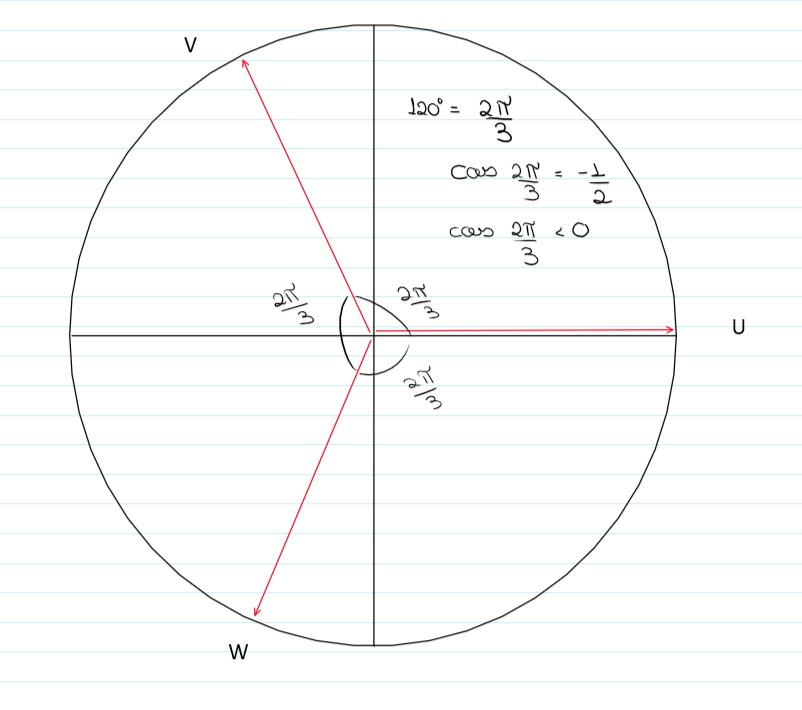
\includegraphics[width=0.5\linewidth]{6.2}
	\caption{A2}
	\label{fig:7}
\end{figure}

\begin{figure}[H]
	\centering
	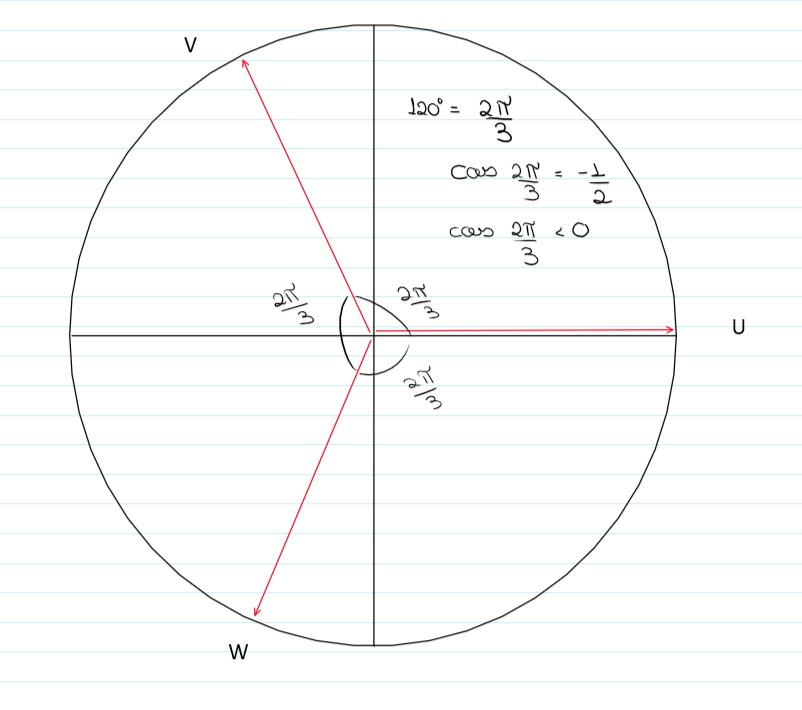
\includegraphics[width=0.5\linewidth]{6.3}
	\caption{A3}
	\label{fig:8}
\end{figure}

\end{sol}


\end{enumerate}
\end{document}